\chapter{保量推荐下的最优广告投放算法}
\label{cha:allocation}

本章我们将提出一种\textit{最优广告投放算法(oPtImal Kwai Advertising, PIKA)},该算法被部署在快手广告平台中的同城页粉丝头条服务中。粉丝头条服务致力于在保证广告主获得其期望的曝光量的情况下,使得广告投放后的总分数最高,其中分数由\ref{eq:score}定义。长达一个月的线上实验表明PIKA的广告投放效果优于目前部署在线上的算法。PIKA算法的核心思想是利用坐标下降法求解一个离线的带约束二次规划问题的KKT条件,该算法分为两个部分:训练模块和投放模块,分别对应线下部分和线上部分。不同于之前所部署的流量控制算法中的硬阈值,PIKA中线下优化所得的对偶变量可以被认为是一种“软阈值”,而算法会根据不同广告的需求投放量和历史数据中的分数给其设置不同的软阈值,进而在满足投放量的同时最大化投放后的总分数。

\section{PIKA算法原理}

\subsection{问题定义}

不妨设$\mathcal{S}$是所有在投广告的集合,它的一个子集$\mathcal{S}_i$第$i$次PV所召回的广告集合,则$\mathcal{S}_i \subset \mathcal{S}$。每个在投广告的总期望曝光量或者说总需求量用$D_j$表示,该广告的投放时长用$T_j$表示。理想情况下,我们希望在投放时长到达$T_j$后,最终的实际广告投放量正好等于$D_j$,因此实际中我们尽量使最终曝光量尽可能接近$D_j$。除此之外,每次PV对于被召回广告的分数也将被用于目标函数。因为对于每次PV只有一小部分广告被召回,因此我们可以用一个稀疏矩阵$\bm{A}$来存储PV对广告的分数,其中$\bm{A}_{ij}$是预测出的第$i$次PV对于第$j$个广告的分数。因此,如果一段时间内有$M$次访问和$N$个在投广告,那么$\bm{A}$应当是一个$M \times N$的矩阵。如果对于第$i$次PV来说,广告$j$没有被召回,则$\bm{A}_{ij}=0$。

最后却也是最重要的,投放矩阵$\bm{X}^{int}$决定每次PV投放哪个广告,即若 $\bm{X}^{int}_{ij} = 1$则将广告$j$投放给PV $i$,否则$\bm{X}^{int}_{ij} = 0$。这是一个\textit{0-1整数规划问题(0-1 Integer Programming Problem)},而且该问题是一个NP-complete问题~\cite{garey2002computers}。为了克服这个困难,我们将投放矩阵松弛为投放概率矩阵$\bm{X}$,它拥有和$\bm{A}$相同的大小,其中$\bm{X}_{ij}$代表将广告$j$投放给PV $i$的概率。为了防止用户体验被广告过多影响,我们要求每次PV只能投放少量广告。如果每次PV最多只能投放1个广告,则
\begin{equation}
\sum_j \bm{X}_{ij} \le 1, \forall i.
\end{equation}
这个约束与概率的归一性(即随机变量所有可能取值的概率之和或概率密度积分等于1)一致,因为不投放广告的概率没有被纳入$\bm{X}$中,而对于PV $i$不投放广告的概率就是$1-\sum_j \bm{X}_{ij}$。每次PV可以投放多个广告的场景将在第\ref{subsec:more_than_one}节中讨论。此外,因为概率的非负性,我们有$\bm{X}_{ij} \ge 0, \forall i,j$。在常见的广告投放算法中,平台从广告主得到的收入小于等于广告日的每日预算是合理的。但是,为了在收入和用户体验之间取得平衡,这里我们将采用等式约束来使广告的最终曝光量等于广告主的需求量。

最后,我们正式用如下优化表达式描述我们的问题:
\begin{equation}
\begin{aligned}
\min_X &-\sum_{i,j} \bm{A}_{ij}\bm{X}_{ij} \\
s.t. & \sum_i \bm{X}_{ij} = \bm{d}_j, \forall j, \\
& \sum_j \bm{X}_{ij} \le 1, \forall i, \\
& \bm{X}_{ij} \ge 0, \forall i, j. 
\label{eq:ori_opt}
\end{aligned}
\end{equation}
$\sum_{j} \bm{A}_{ij}\bm{X}_{ij}$是PV $i$的分数的期望,因此目标函数$\sum_{i,j} \bm{A}_{ij}\bm{X}_{ij}$的含义就是所有PV的期望分数的总分数。为了与优化问题的标准格式一致,我们最小化目标函数的负值,而且由于它是一个线性函数,因此正负号不影响凹凸性。注意到,上式中的需求量符号是$\bm{d}_j$而不是$D_j$,这里$\bm{d}_j$代表训练周期内的期望需求量。作为一个简单的例子,对于广告$j$来说,如果当前客户端展示量,或者说曝光量,是$\bm{c}_j$,剩余投放时长是$\bm{t}_j$,训练周期是$T_p$(即每隔$T_p$求解一次上述优化问题),则$\bm{d}_j$可以用如下公式计算:
\begin{equation}
\bm{d}_j = \frac{D_j - \bm{c}_j}{\bm{t}_j}T_{p}. \label{eq:avg}
\end{equation}
平滑投放通过上式里把总需求量均匀分散于投放时长内的所有训练周期被隐式的实现了,不过真实环境中流量是有高峰和低谷的,一个线上可用的需求量分配方案将在第\ref{subsec:hourly_d}节中被详细介绍。

这是一个标准的带约束的\textit{线性规划问题(Linear Programming problem, LP)},而且已经有很多成熟的解法。但是,简单的给出最优解$\bm{X}$并不适用于我们的场景,因为我们所需要的是一个等式来指导线上广告投放,从而当被召回广告及其分数可用时我们可以迅速给出投放概率。而如果只是简单的算出最优$\bm{X}$,这也只是历史数据的最优解,无法用于未来PV的广告投放。通过在目标函数里加入$\bm{X}$的二次项可以得到关于$\bm{X}$和对偶变量的等式。此外,由于噪声的存在以及预测分数$\bm{A}$的抖动,如果直接优化$\sum_{i,j} \bm{A}_{ij}\bm{X}_{ij}$可能会导致过拟合和求解结果不稳定。另一个出发点是,$\bm{X}$中的非零值元素比较分散的情况应该好于非零值集中在少数几个元素,因为前者对于分数$\bm{A}$的变化不敏感。因此,我们在\eqref{eq:ori_opt}的基础上加入正则项:
\begin{equation}
\begin{aligned}
\min_X &\sum_{i,j}  (-\bm{A}_{ij}\bm{X}_{ij} + \frac{\lambda}{2}{\bm{X}_{ij}}^2) \\
s.t. & \sum_i \bm{X}_{ij} = \bm{d}_j, \forall j, \\
& \sum_j \bm{X}_{ij} \le 1, \forall i, \\
& \bm{X}_{ij} \ge 0, \forall i, j, 
\label{eq:opt}
\end{aligned}
\end{equation}
其中$\lambda$是正则化系数。

\eqref{eq:opt}将在线下求解之后用于指导线上投放,因此我们的算法可以分为两部分:训练模块和投放模块。

\subsection{训练模块} \label{subsec:train}

在训练之前,服务器会为训练收集历史数据。之后求解优化问题\eqref{eq:opt}。显然,\eqref{eq:opt}是一个凸优化问题,意味着满足KKT条件的解就是优化问题的最优解。对于$\forall i,j$,\eqref{eq:opt}的KKT条件是:
\begin{equation}
\begin{aligned}
\sum_i{\bm{\hat{X}}_{ij}} - \bm{d}_j &= 0, \\
\sum_j{\bm{\hat{X}}_{ij}} -1 &\le 0, \\
\bm{\beta}_i &\ge 0, \\
\bm{\beta}_i\sum_j \bm{\hat{X}}_{ij} &= 0, \\
-\bm{\hat{X}}_{ij} &\le 0, \\
\bm{\Gamma}_{ij} &\ge 0, \\
\bm{\Gamma}_{ij}\bm{\hat{X}}_{ij} &= 0, \\
-\bm{A}_{ij} + \lambda\bm{\hat{X}}_{ij} + \bm{\alpha}_j + \bm{\beta}_i - \bm{\Gamma}_{ij} &= 0, \\ 
\label{eq:kkt}
\end{aligned}
\end{equation}
其中$\bm{\hat{X}}$是理论上的最优解,$\bm{\alpha}, \bm{\beta}$和$\bm{\Gamma}$分别是对应\eqref{eq:opt}中的三个约束的对偶变量。由\eqref{eq:kkt}可以发现$\bm{\hat{X}}_{ij}$ 和 $\bm{\Gamma}_{ij}$二者至少有一个必须等于0,再加上$\bm{X}_{ij} \ge 0$的约束,我们可用下式表示$\bm{\hat{X}}_{ij}$:
\begin{equation}
\bm{\hat{X}}_{ij} = \max\{0, \frac{1}{\lambda} (\bm{A}_{ij} - \bm{\alpha}_j - \bm{\beta}_i)\}, \forall i, j. 
\label{eq:xeq}
\end{equation}
将上式带回\eqref{eq:kkt}中,则可以改写为:
\begin{equation}
\begin{aligned}
\sum_i{\bm{\hat{X}}_{ij}} - \bm{d}_j &= 0, \\
\sum_j{\bm{\hat{X}}_{ij}} - 1 &\le 0, \\
\bm{\beta}_i &\ge 0, \\
\bm{\beta}_i\sum_j \bm{\hat{X}}_{ij} &= 0, \\
\bm{\hat{X}}_{ij} - \max\{0, \frac{1}{\lambda} (\bm{A}_{ij} - \bm{\alpha}_j - \bm{\beta}_i)\} &= 0. \\ 
\end{aligned}
\end{equation}
这样就已经减少到2个对偶变量了,而且其中一个还是对应等式约束的对偶变量,即$\bm{\alpha}$。因此,我们可以利用坐标下降法获得最优解,其中$\bm{\alpha}$和$\bm{\beta}$依次被优化并迭代,直到到达停止迭代判据或者迭代次数。因为$\bm{\alpha}$对应等式约束,因此在计算$\bm{\alpha}_j$时可以固定住$\bm{\beta}$,并行的解算,使得 $\sum_i{\bm{\hat{X}}_{ij}} - d_j = 0$。至于计算$\bm{\beta}$,可以先将其全部设为0,如果$\sum_j{\bm{\hat{X}}_{ij}} \le 1$,则继续令$\bm{\beta}_i=0$;否则并行的计算$\bm{\beta}_i$使得$\sum_j{\bm{\hat{X}}_{ij}} = 1$。算法\ref{alg:offline}完整的描述了离线最优解算法。

\begin{algorithm}[tb]
	\caption{离线最优解算法} 
	\label{alg:offline}
	\begin{algorithmic}[1]
		\REQUIRE 分数矩阵 $\bm{A}$, 需求量 $\bm{d}$, 在投广告数 $M$, 上一个周期内的访问数 $N$, 收敛界 $b$
		\ENSURE 对偶变量 $\bm{\alpha}$ 
		\STATE 初始化: $\bm{\beta}_i \leftarrow 0$ for all $i$, $\bm{\alpha}_j \leftarrow 0$, $\bm{\alpha}^{old}_j \leftarrow 1$ for all $j$
		\WHILE{${\left\| \bm{\alpha}^{old} - \bm{\alpha} \right\|}$ > 停止判据 \&\& 迭代步数 < 步数阈值} 
		\FOR{$i < N$}
		\IF{$\sum_j \bm{X}_{ij} \le 1$}
		\STATE $\bm{\beta}_i \leftarrow 0$
		\ELSE
		\STATE 求解 $\bm{\beta}_i$ s.t. $\sum_j \bm{X}_{ij} = 1$ \label{solve_beta}
		\ENDIF
		\ENDFOR
		\FOR{$j < M$}
		\STATE 求解 $\bm{\alpha}_j$ s.t. $\sum_i \bm{X}_{ij} = \bm{d}_j$ \label{solve_alpha}
		\IF{$\bm{\alpha}_j < b$}
		\STATE 广告 $j$ 无解而且不会参与后续迭代的计算 \label{bound}
		\ENDIF
		\ENDFOR
		\STATE $\bm{\alpha}^{old} \leftarrow \bm{\alpha}$
		\ENDWHILE
		\RETURN $\bm{\alpha}$ 
	\end{algorithmic}
\end{algorithm}

算法\ref{alg:offline}中的$\bm{X}_{ij}$均由\eqref{eq:xeq}计算。$\bm{X}$的求和其实是一个分段折线函数,因此我们可以用二分法来实现算法\ref{alg:offline}中的求根操作(第\ref{solve_alpha}行和第\ref{solve_beta}行)。这里的$\bm{\alpha}$可以被认为是一种“软阈值”:当$\bm{A}_{ij} \le \bm{\alpha}_j$时,广告$j$不可能被投放给PV $i$;当$\bm{A}_{ij} > \bm{\alpha}_j$时,$\bm{A}_{ij}$越大则广告$j$被投放给PV $i$的概率越大。因此在某种程度上说,$\bm{\alpha}$揭露了广告$j$的分数和它的需求量之间的某种关系。

然而,简单的交替求解$\bm{\alpha}$和$\bm{\beta}$或者说坐标下降可能会因为一些广告无解的情况存在而整体不收敛。比如,当一个广告在上一个训练周期内的召回量太少甚至少于需求量时,这个广告是无解的。一种可能的解决方案是像SHALE~\cite{bharadwaj2012shale}一样,在我们的优化表达式中加一个惩罚项:
\begin{equation}
\begin{aligned}
\min_X &\sum_{i,j}  (-\bm{A}_{ij}\bm{X}_{ij} + \frac{\lambda}{2}{\bm{X}_{ij}}^2) + \sum_j \bm{p}_j\bm{u}_j  \\
s.t. & \sum_i \bm{X}_{ij} + \bm{u}_j = \bm{d}_j, \forall j, \\
& \sum_j \bm{X}_{ij} \le 1, \forall i, \\
& \bm{X}_{ij} \ge 0, \bm{u}_j \ge 0. \forall i, j. 
\end{aligned}
\end{equation}
但是,这种方法会增加计算复杂度,而且引入了另一个需要调节的超参数$\bm{p}$。因为快手的召回系统机制可以确保没有一个广告会一直召回量不足,因此我们可以简单的放弃在下个周期通过上述正常方式投放该广告。我们设置了一个界限$b$,当迭代过程中$\bm{\alpha}_j$比$b$还小,该广告$j$就会被认为是无解的,并不会参与本周期的后续迭代计算。只设置下界$b$的原因是$\bm{\alpha}$其实存在一个隐式的上界,这个值是一个跟该广告分数和需求量相关的值。而一旦一个广告召回量太少,迭代过程中$\bm{\alpha}_j$就会一直减小,最终触发下界停止迭代。无解的广告无法通过下一小节将要介绍的正常的投放模块投放出去,而这些广告的投放方法将在第\ref{subsec:guarantee}节中讨论。

$\bm{\alpha}$是投放模块唯一需要从训练模块获得的参数,因此训练模块只需返回$\bm{\alpha}$即可。

\subsection{投放模块}

首先,假设线上数据和线下数据完全相同,那么在训练模块计算出$\bm{\alpha}$之后,每当一个PV到来,它的广告投放概率向量可以根据\eqref{eq:xeq}求得。算法\ref{alg:online}详细描述了线上投放算法的具体步骤。该算法将输出对于该次PV来说的广告投放概率向量$\bm{p}$,之后我们将根据$\bm{p}$对广告进行采样,被选中的广告就会被投放给该次PV。请注意,不投放广告的概率是 $1-\sum_j \bm{p}_j$。最后,因为这里我们假设线上数据和线下数据完全相同,因此该算法的最终分数一定和线下计算的最优解相同。

\begin{algorithm}[tb]
	\caption{线上投放概率算法} 
	\label{alg:online}
	\begin{algorithmic}[1]
		\REQUIRE 一次PV的分数向量 $\bm{s}$, 广告的需求量 $\bm{d}$, 对偶变量 $\bm{\alpha}$, 线下可解广告数 $M$  (只有可解广告才会通过该算法投放)
		\ENSURE 投放概率向量 $\bm{p}$
		\STATE 初始化: $\beta \leftarrow 0$
		\FOR{$j < M$}
		\STATE $\bm{p}_j \leftarrow \max \{0, \frac{1}{\lambda}  (\bm{s}_j - \bm{\alpha}_j - \beta )\}$
		\ENDFOR
		\IF{$\sum_j \bm{p}_j > 1$}
		\STATE 求解 $\beta$ s.t. $\sum_j \bm{p}_j = 1$
		\FOR{$j < M$}
		\STATE $\bm{p}_j \leftarrow \max \{0, \frac{1}{\lambda}  (\bm{s}_j - \bm{\alpha}_j - \beta )\}$
		\ENDFOR
		\ENDIF
		\RETURN $\bm{p}$
	\end{algorithmic}
\end{algorithm}

在实际情况下,虽然线上数据并不能和线下数据完全相同,但是在线下数据和线上数据独立同分布的假设成立的前提下,我们的算法也能取得较好的效果,因为$\bm{\alpha}_j$其实在某种程度上可以被认为是广告$j$分数的分位数。而且训练模块和投放模块之间的时间间隔很短(在我们的实现方法中这个间隔是5min,即新数据每5min替换一次旧数据),因此线下数据和线上数据的分数的统计特征不会发生剧烈变化。此外,一切前人的工作也已经从理论上分析了这个问题~\cite{devanur2009adwords, feldman2010online}。

\section{工程实现细节}

上述的PIKA算法是基于概率的而不是确定的投放计划,因此可能出现真实曝光量跟需求量相去甚远的情况。除此之外,限制一个PV最多只能投放一个广告可能会严重限制我们的算法的适用性。最后,简单的将总需求量均匀的摊分入投放时段内的训练周期内不是一个好的机制,因为流量会在白天和夜晚剧烈变换。在这一节,我们将逐一提出方案缓解上述问题。

\subsection{曝光量保底策略} \label{subsec:guarantee}

正如第\ref{subsec:train}节中所提到的,因为召回量不足等问题会导致部分广告在训练模块中无解,而这些广告是无法通过上文所提出的正常的投放模块投放出去的。除此之外,简单的依靠上述算法是不能保证最终曝光量正好等于需求量的,因为线下数据和线上数据并不相同。我们需要提出一种机制使得曝光量尽可能接近广告主的需求量。

我们设计一种\textit{兜底投放策略}来投放在训练模块中无解的广告和即将结束投放的广告。该策略可以分为三步:
\begin{enumerate}
	\item 检查对于该次PV是否已经有广告通过正常的投放模块被投放,如果没有则进行下述步骤,否则曝光量保底策略不投放视频;
	\item 收集上一个训练周期无解的广告和即将结束投放却还未满足需求量的广告;
	\item 从上述广告集合中选取一个广告。\label{select}
\end{enumerate}

上述第\ref{select}步的选取操作可以因地制宜,我们的策略是选取一个排序分数最大的视频,不过注意,这里的排序分数和分数矩阵$\bm{A}$中的分数不完全相同。如果一个广告没有即将结束投放,它的排序分数就是它原来在$\bm{A}$中的分数;否则,它的分数将被饥渴度替代,其中饥渴度($hd$)
由下式计算:
\begin{equation}
	hd = 1 + \frac{left\_demand}{left\_time}.
\end{equation}
因为原来在$\bm{A}$中的分数均小于1,因此我们的策略相当于给即将结束投放的广告更高的优先级。在我们的实现中,距离结束投放的时间少于15min被认为是“紧急广告”,它们的排序分数将使用饥渴度。

最后,一个广告的召回量可能会在相邻的两个训练周期内剧烈变化。比如,在该广告投放的初始阶段,由于冷启动等问题,该广告的召回量会比正常水平低得多。然而训练模块把这个当成了正常水平,因此如果在投放周期内召回量恢复正常,那么服务器就会投放次数过多。为了防止投放数量超过需求量太多,当一个广告在投放周期内的投放量已经超过其训练模块中周期需求量$\bm{d}_j$的两倍时,该广告将会在该投放周期内停止投放。

\subsection{投放多于一个广告} \label{subsec:more_than_one}

上一小节的讨论中,我们限制了一次PV最多只能投放一个广告,这将严重限制PIKA算法的通用性。针对这个问题,有两种方案来解决:\textit{无放回采样}和\textit{将$\bm{X}$看做期望}。
\begin{enumerate}[1)]
	\item \textbf{无放回采样}
	
	这种方法在数学上严谨但是很难实现,因为计算复杂度太高。假设$\bm{v}$是一个代表在单次采样操作中广告被采样概率的向量,同时每次PV最多可以投放2个广告,即对于每次PV我们应当进行两次无放回采样。因此,广告$j$被采样,或者说被投放,的概率就是
	\begin{equation}
	\bm{p}_j = \bm{v}_j + \sum_{i \ne j}\bm{v}_i\frac{\bm{v}_j}{1 - \bm{v}_i}, \forall j.
	\label{eq:no_replace}
	\end{equation}
	作为对比,在最多只能投放1个广告的情况下,采样概率就是简单的$\bm{p}_j = \bm{v}_j$。更严重的是,\eqref{eq:no_replace}使得$\bm{\alpha}$中的元素变得彼此相关,或者说耦合,因此$\bm{\alpha}$无法像之前那样并行计算。而且这还只是最多投放2个广告的情况,泛化的场景将使得这种方案变成灾难。
	
	\item \textbf{将$\bm{X}$看作期望}
	
	如果我们将$\bm{X}$看作期望而不是概率,原本的约束可以简单的被替换为:
	\begin{equation}
	\begin{aligned}
	\sum_j{\bm{X}_{ij}} \le 1 &\Rightarrow \sum_j{\bm{X}_{ij}} \le m, \forall i, \\
	\bm{X}_{ij} \ge 0 &\Rightarrow 0 \le \bm{X}_{ij} \le 1, \forall i, j. 
	\end{aligned}
	\end{equation}
	这些约束代表着每次PV最多可以投放$m$个广告,同时每个广告最多投放一次。之前,$\bm{X}_{ij} \le 1$是被隐式的约束着,因为在$\sum_j{\bm{X}_{ij}} \le 1$的情况下这个约束自然满足。这种方案的训练模块和算法\ref{alg:offline}一样,除了$\bm{X}$的公式需要换成:
	\begin{equation}
	\bm{X}_{ij} =\min\{1, \max\{0, \frac{1}{\lambda} (\bm{A}_{ij} - \bm{\alpha}_j - \bm{\beta}_i)\}\}, \forall i, j. 
	\end{equation}
	除此之外,算法\ref{alg:offline}里的$\sum_j{\bm{X}_{ij}} \le 1$ 和 $\sum_j{\bm{X}_{ij}} = 1$应改为$\sum_j{\bm{X}_{ij}} \le m$ 和 $\sum_j{\bm{X}_{ij}} = m$。
	
	但是,这种方案的困难之处出现在投放模块。算法\ref{alg:online}所得的$\bm{p}$不再代表概率,因此在采样时不能简单的依照$\bm{p}$。如果一个广告允许被投放于同一次PV两次,我们可以将$\bm{p}$简单的分成$m$个子序列(允许将一个元素一分为二),其中每一个子序列之和小于等于1。我们很容易就可以保证$\bm{p}$中的元素最多只被切分一次。之后,根据这些$m$个期望,进行$m$次加权采样。在附录中我们将证明采样的期望和$\bm{p}$一样。为了更形象的说明我们的做法,举如下一个例子:假如$\bm{p} = [0.5, 0.6, 0.7]$,$m=2$。则$\bm{p}$可以被分成$\bm{p}^1 = [0.5, 0.5]$和$\bm{p}^2 = [0.1, 0.7]$,其中0.6被分成了0.5和0.1。之后,分别根据$\bm{p}^1$和$\bm{p}^2$采样两次,得到投放的广告。但实际情况是给一次PV投放两次相同的广告是不允许的,因此该方法会导致广告$j$的实际采样期望小于$\bm{p}_j$。还以刚才的$\bm{p}$为例,如果广告$2$已经根据$\bm{p}^1$被采样了,则$\bm{p}^2$就会变成$\bm{p}^2 = [0.7]$。显然,只有在划分$m$块的操作中被切分的$\bm{p}_j$会受到影响,而且受影响的广告的数量最多是$m-1$,这远小于在投广告的数量。再考虑到广告是被随机地切分而且曝光量保底策略可以保证最终的曝光量,这个解决方案相比前一个可用性大大提升。
	\end{enumerate}

\subsection{小时需求量} \label{subsec:hourly_d}

在\eqref{eq:avg}中,周期需求量$\bm{d}$通过将总需求量均匀的分摊入投放时段内的训练周期内获得。但是很显然页面访问流量会在白天和夜晚呈现出巨大差别,因此由\eqref{eq:avg}得到的$\bm{d}$将会在流量高峰时太少而在流量低谷处又太多。我们使用一种\textit{小时需求量}策略来拟合流量的趋势。广告$j$的总需求量$D_j$根据其投放周期内不同小时的权重被分配到各个小时内,其中权重是一个拟合各个小时流量的经验值。举例来说,假设一个广告的总需求量是30,投放时长是3h。同时,这三个小时的权重是$\bm{w} = [4, 5, 6]$。那么这三个小时内的期望投放量就是$\bm{e} = [8, 10, 12]$。不过,每经过一个小时就会重新分配一次。假设$\bm{e}_j$是在该小时结束时期望的曝光量,$\bm{c}_j$是当前曝光量,$\bm{h}_j$是直到当前小时结束的剩余时间,$T_p$是训练周期。那么最终的当前周期小时需求量$\bm{d}_j$就是:
\begin{equation}
\bm{d}_j = T_{p}\frac{\bm{e}_j - \bm{c}_j}{\bm{t}_j}, \forall j.
\end{equation}
从某种程度上,小时需求量策略也使得投放更平滑。如果投放频率低于预期,那么在当前小时结束前$\bm{d}_j$就会增大;反之,如果投放频率高于预期,则$\bm{d}_j$就会减小甚至变为0。

\section{实验与结果}

我们首先进行了仿真实验以验证PIKA算法的可行性,之后部署到线上并和之前部署的算法进行对比。

\subsection{仿真实验}

为了简单起见,我们从快手的数据库中提取了某个时间段内的所有页面访问,并按照时序划分为训练集和测试集,各有50万次PV。同时,我们选取400个广告投放,各有50的需求量。这里我们就不再引入召回机制,而是直接用预测服务器计算所有PV对这400个广告的点击率(Click-Through Rate, CTR),即$\bm{A}$中的分数就是CTR。在仿真实验中只有训练模块和正常的投放模块被实现了,即仿真中没有曝光量保底策略。此外,投放模块中计算出投放概率$\bm{p}$后没有后续的采样,而是把期望当做投放量。所有已投放广告的预测CTR之和被当做目标函数。

\begin{figure}[tb]
	\centering
	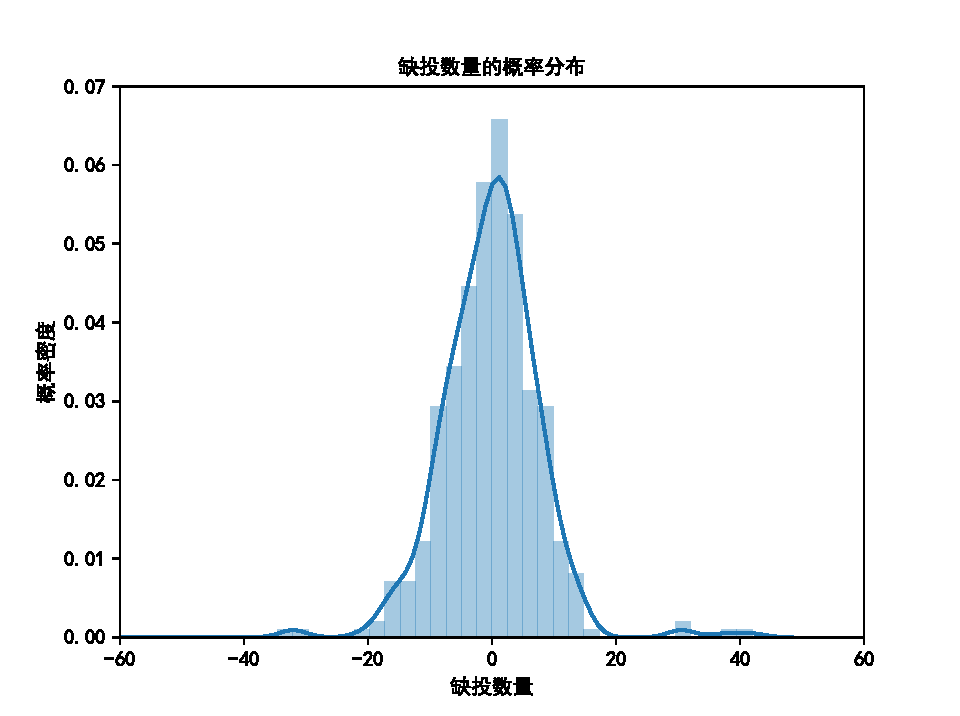
\includegraphics[width=\textwidth]{simulation.pdf}
	\caption{仿真实验中测试数据集的缺投情况统计。训练数据和测试数据各有50万次PV,同时有400个广告均有50的需求量。这个缺投量的分布和高斯分布非常相似,其中$\mu = -0.49$,$\sigma = 9.41$。}
	\label{fig:delivery}
\end{figure}

图\ref{fig:delivery}是这400个广告投放完成后对缺投量的统计。其中x轴的分辨率是3,正数代表缺投,负数代表超投。y轴是广告落入每个桶内的数量。这个分布非常像高斯分布,其中$\mu = -0.49$,$\sigma = 9.41$,而这个现象也与中心极限定理一致。测试集的需求量之和是20,000,实际投放量之和是21,219。最后,训练集的平均CTR=35.93\%,测试集平均CTR=35.85\%。作为对比,简单贪心法的平均CTR=27.80\%,即PIKA算法相对提升了29.0\%。

从仿真实验的结果中我们可以总结出:
\begin{itemize}
	\item PIKA的投放量的期望是可以满足需求量的,而且缺投量近似服从零均值高斯分布。这个特点侧面证明了曝光量保底策略的必要性,因为正常的投放模块只能保证投放量的期望满足需求,而实际中我们必须满足广告主的需求;
	\item PIKA算法可以在训练模块和投放模块取得近似相同的投放效果,侧面证明PV的统计特征不会在短时间内剧变,以及我们的算法适用于当前场景。而且,相比于简单贪心法,PIKA可以在投放效果方面带来明显的改进。
\end{itemize}

仿真实验已经印证了PIKA算法的可用性及其性能,后续我们将算法部署到快手同城页的粉丝头条服务上,通过实际投放广告检验算法性能与效果。

\subsection{线上实验设置}

我们在快手平台上开展了为期一个月的实验来验证PIKA算法带来的改进。PIKA被部署在快手的同城页粉丝头条服务中,在这里广告的召回是基于访问者与广告主之间的定位。每当一次PV到来,它会被随机地分到四组服务器其中的一组。同时,每个广告的总需求量也被均匀地分成四份,每一组服务器需要独立的保证各自的需求量得到满足。这套机制在快手被称作“预算隔离”,这是一种A/B测试的实现方式,提供了一个高效的实验环境以验证、对比新算法和当前部署算法的性能与效果。在实验期间,这四组中有一组部署了PIKA算法,其余三组都是原先的FC算法。实验组除了将FC替换为PIKA之外,其余的上下游服务都和对照组一样。

 PIKA算法中有一些需要提前设置好的超参数,比如正则化系数$\lambda$,训练周期$T_p$和收敛边界$b$:
 \begin{itemize}
 	\item 正则化系数$\lambda$。\eqref{eq:xeq}描述了$\bm{X}$和$\lambda$之间的关系。结合\eqref{eq:opt}来分析,$\lambda$太大会导致投放概率主要受需求量$\bm{d}$的影响而不是分数$\bm{A}$。但是,如果$\lambda$太小,则会迫使$\bm{\alpha}_j$很接近广告$j$在该训练周期内的最大分数,从而导致算法不稳定,因为最大分数会经常变化剧烈而且求最大值的操作对噪声敏感。根据粗略的实验,我们最终将$\lambda$设置为一个接近被投放广告平均分数的值。
 	\item 训练周期$T_p$。虽然较小的$T_p$可以确保$\bm{\alpha}$被经常更新并且减少因为存储历史数据所占用的内存,但是数据不足的话会导致$\bm{\alpha}$不稳定。反之,较大的$T_p$虽然可以令$\bm{\alpha}$比较稳定,但是也会使得$\bm{\alpha}$时效性变差而且占用大量内存。经过权衡,我们最终将$T_p$设为5min。
 	\item 收敛边界$b$。这个参数是用来判断一个广告是否可解,而且通过上文的分析我们已经知道只需要设置下界即可。在我们的实现中,$b$被设为-1,即如果$\bm{\alpha}_j<-1$则广告$j$就被认为是无解的。
 \end{itemize}

\subsection{关键指标}

曝光量是最重要的指标之一,实际曝光量应当多于广告主的需求量但又不能超过太多。如果广告的最终曝光量在需求量的上下5\%范围内,就认为是正常完成了投放;否则被标记为缺投或者超投。

除此之外,主要有4个投放效果相关的优化指标:关注率(Follow Rate, FTR)、点击率(Click-Through Rate, CTR)、点赞率(Like Rate, LTR)和点踩率(Hate Rate, HTR)。如果一个访问用户被投放了一个广告,之后他/她关注了作者、点击了广告、给广告点赞或者给广告点踩,则会被算作一次关注、点击、点赞或者点踩。当广告投放结束时,总的关注量、点击量、点赞量和点踩量除以总的曝光量就是关注率、点击率、点赞率和点踩率。

训练耗时和线上反馈延迟也都是重要的指标,这些指标决定了我们的算法是否能够真正在线上使用。

\subsection{线上实验结果}

在每个训练周期内,单台服务器的访问量大概在$10^5$到$10^6$的量级,在投广告数大概在$10^5$量级。页面访问数,即$\bm{A}$的行数,和总需求量$\bm{d}$的比值大概在$5:1$左右。

我们的PIKA算法部署在56核CPU的服务器上,其中每个CPU核是Intel (R) Xeon (R) CPU E5-2680 v4 @ 2.40GHz。训练时迭代100次耗时小于6s,与之对应的是训练周期为300s。同时,线上的反馈延迟平均小于0.2ms。

在曝光量方面,超投广告的数量小于一天总广告数量的0.1\%,缺投广告数量则小于0.15\%。这些曝光量相关的指标,PIKA表现与FC大致相同,因此可以说PIKA算法是能够保证投放量的。

因为在训练阶段可能会存在一些广告无解的情况,因此有必要统计无解订单的数量。在单个训练周期内,最多只有5\%的广告不可解,而且这些无解广告在不同训练周期内频繁变化,也就是说几乎没有广告会在其整个投放时段内一直都是无解的状态。但是,在快手的粉丝头条服务中有一类被称作“商业定向”的广告服务,需要广告主设定一些目标客户的属性,比如年龄等。如果这些目标设定的太详细而需求量却很大,广告的召回量就会被迫减少甚至比需求量还少,这就会使得该广告一直无解。幸运的是,这类广告只占总广告数量不足0.1\%,而这些都是包括在上一段的缺投统计中的。

\begin{figure}[tb]
	\centering
	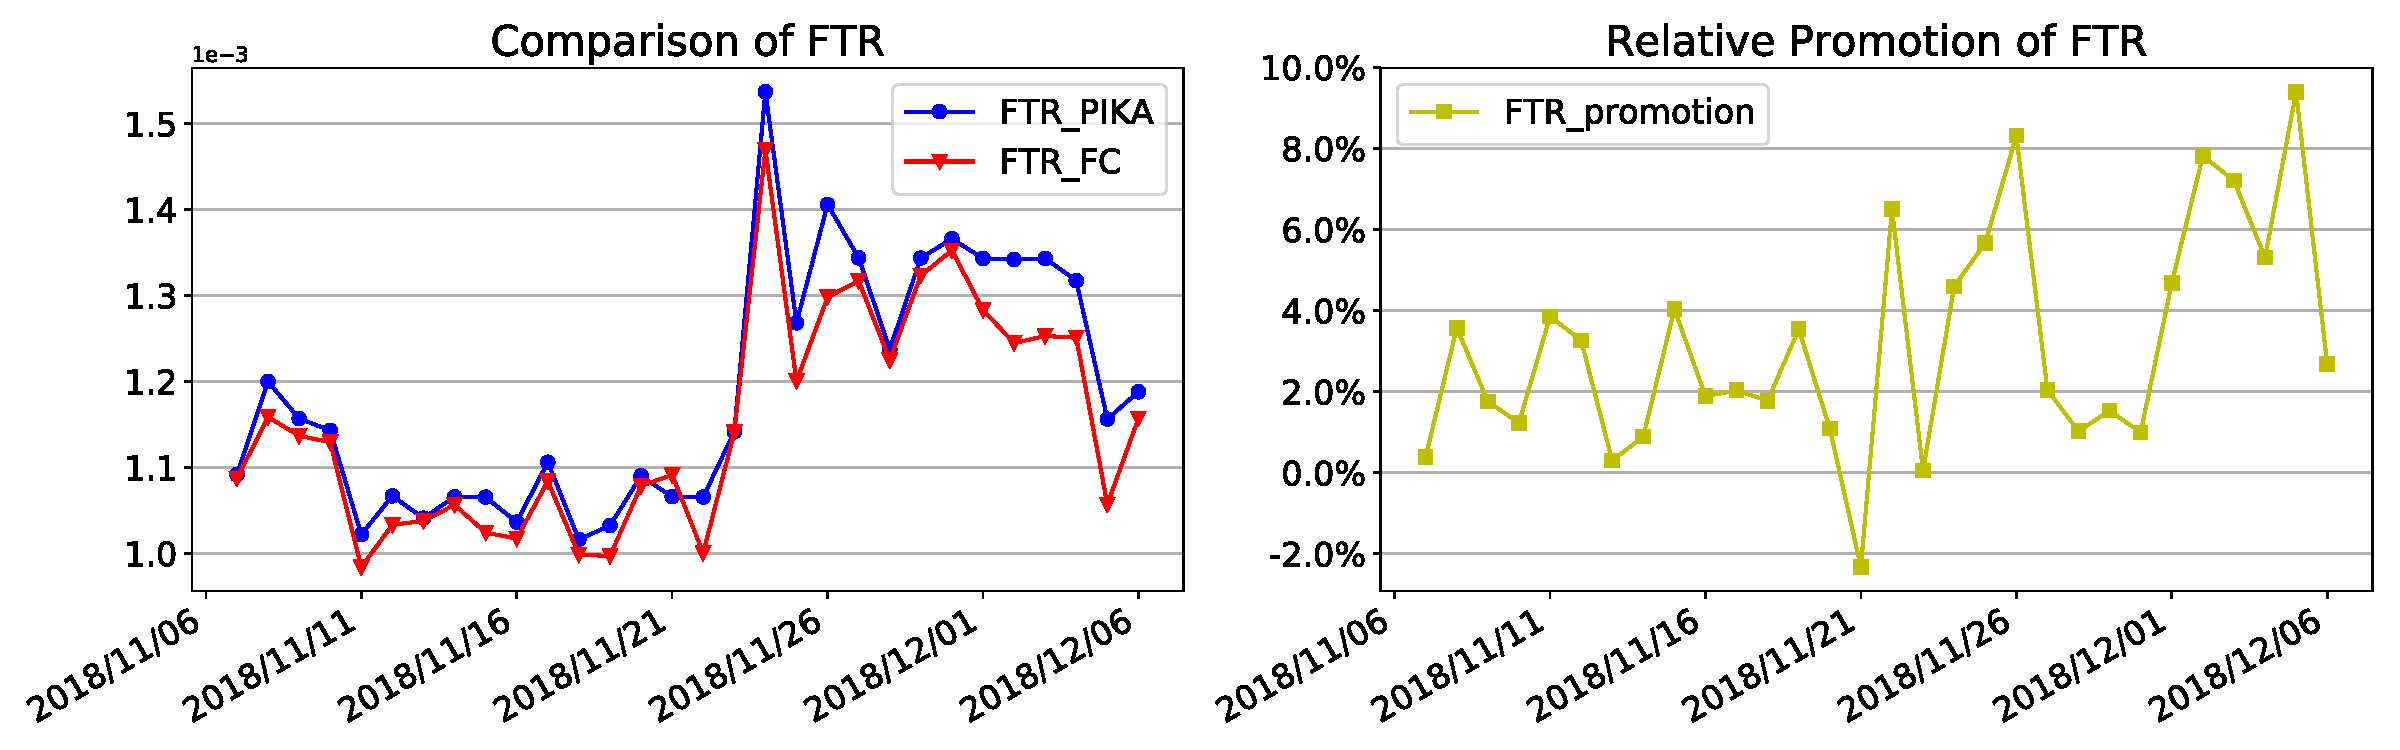
\includegraphics[width=\textwidth]{FTR.pdf}
	\caption{PIKA算法和FC在一个月内的FTR比较以及相对提升。除了一天之外(2018/11/21),PIKA的FTR均高于FC的。相比于FC,PIKA的FTR平均提升了$+3.48\%$。}
	\label{fig:FTR}
\end{figure}

\begin{figure}[tb]
	\centering
	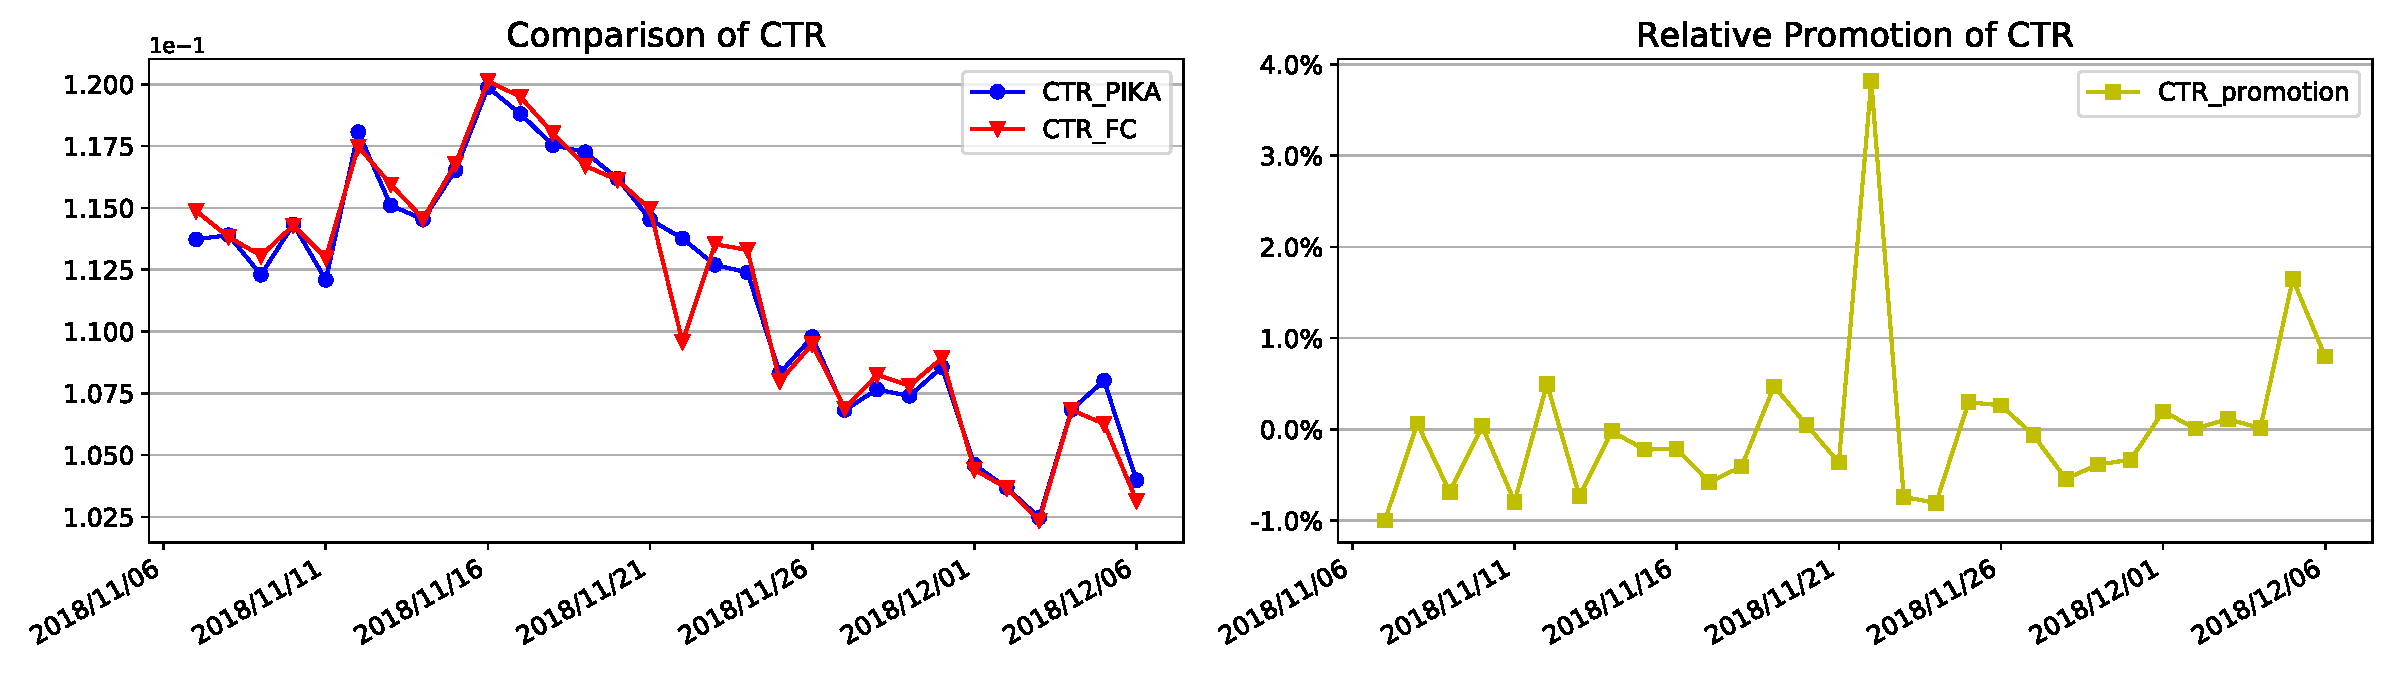
\includegraphics[width=\textwidth]{CTR.pdf}
	\caption{PIKA算法和FC在一个月内的CTR比较以及相对提升。PIKA和FC的CTR在实验期间没有明显区别,而且最终的平均CTR,PIKA只相对提升了$+0.0446\%$,可以忽略不计。}
	\label{fig:CTR}
\end{figure}

PIKA和FC在投放效果指标上的比较以及相对提升展示在图\ref{fig:FTR}到\ref{fig:HTR}中,分别对应FTR、CTR、LTR和HTR。左子图中的蓝色圆形线代表着PIKA的指标,红色倒三角线代表着FC的指标。右子图中的黄色圆形线代表着PIKA相比于FC的相对提升。理想结果是PIKA的FTR、CTR和LTR均高于FC,而PIKA的HTR低于FC。但是,实际结果是PIKA的FTR除了一天之外,均高于FC。二者的CTR和LTR没有明显区别,而PIKA的HTR比FC稍微低一些。在这四种指标上,一个月以来的总的相对提升幅度是:\textbf{FTR $+3.476\%$, CTR $+0.04463\%$, LTR $+0.7522\%$, HTR $-1.104\%$}。虽然在\eqref{eq:score}中,分数是FTR和CTR的组合,但是FTR被给予的更高的权重,因为我们认为FTR更重要。LTR和HTR是次要指标,其实是以某种方式隐式地与FTR和CTR关联着。所以,PIKA在最重要的,或者主要优化的,指标上(FTR)优于FC,在其他指标上几乎没有明显区别,因此可以得出结论:在我们的实验中PIKA的表现优于FC。而且,FC在快手经过了将近一年的调试获得了稳定和良好的效果,但是PIKA在上线测试之前仅仅调试了几次而已,因此或许还存在一些改进空间。最后,线上实验中PIKA的提升效果不如仿真实验中提升那么明显是因为仿真实验中的基准是简单贪心法,而不是FC。除此之外,仿真中采用的评价指标是预测CTR之和,而不是真实的CTR,由预测分数带来的偏差和方差也会影响实验结果。

\begin{figure}[tb]
	\centering
	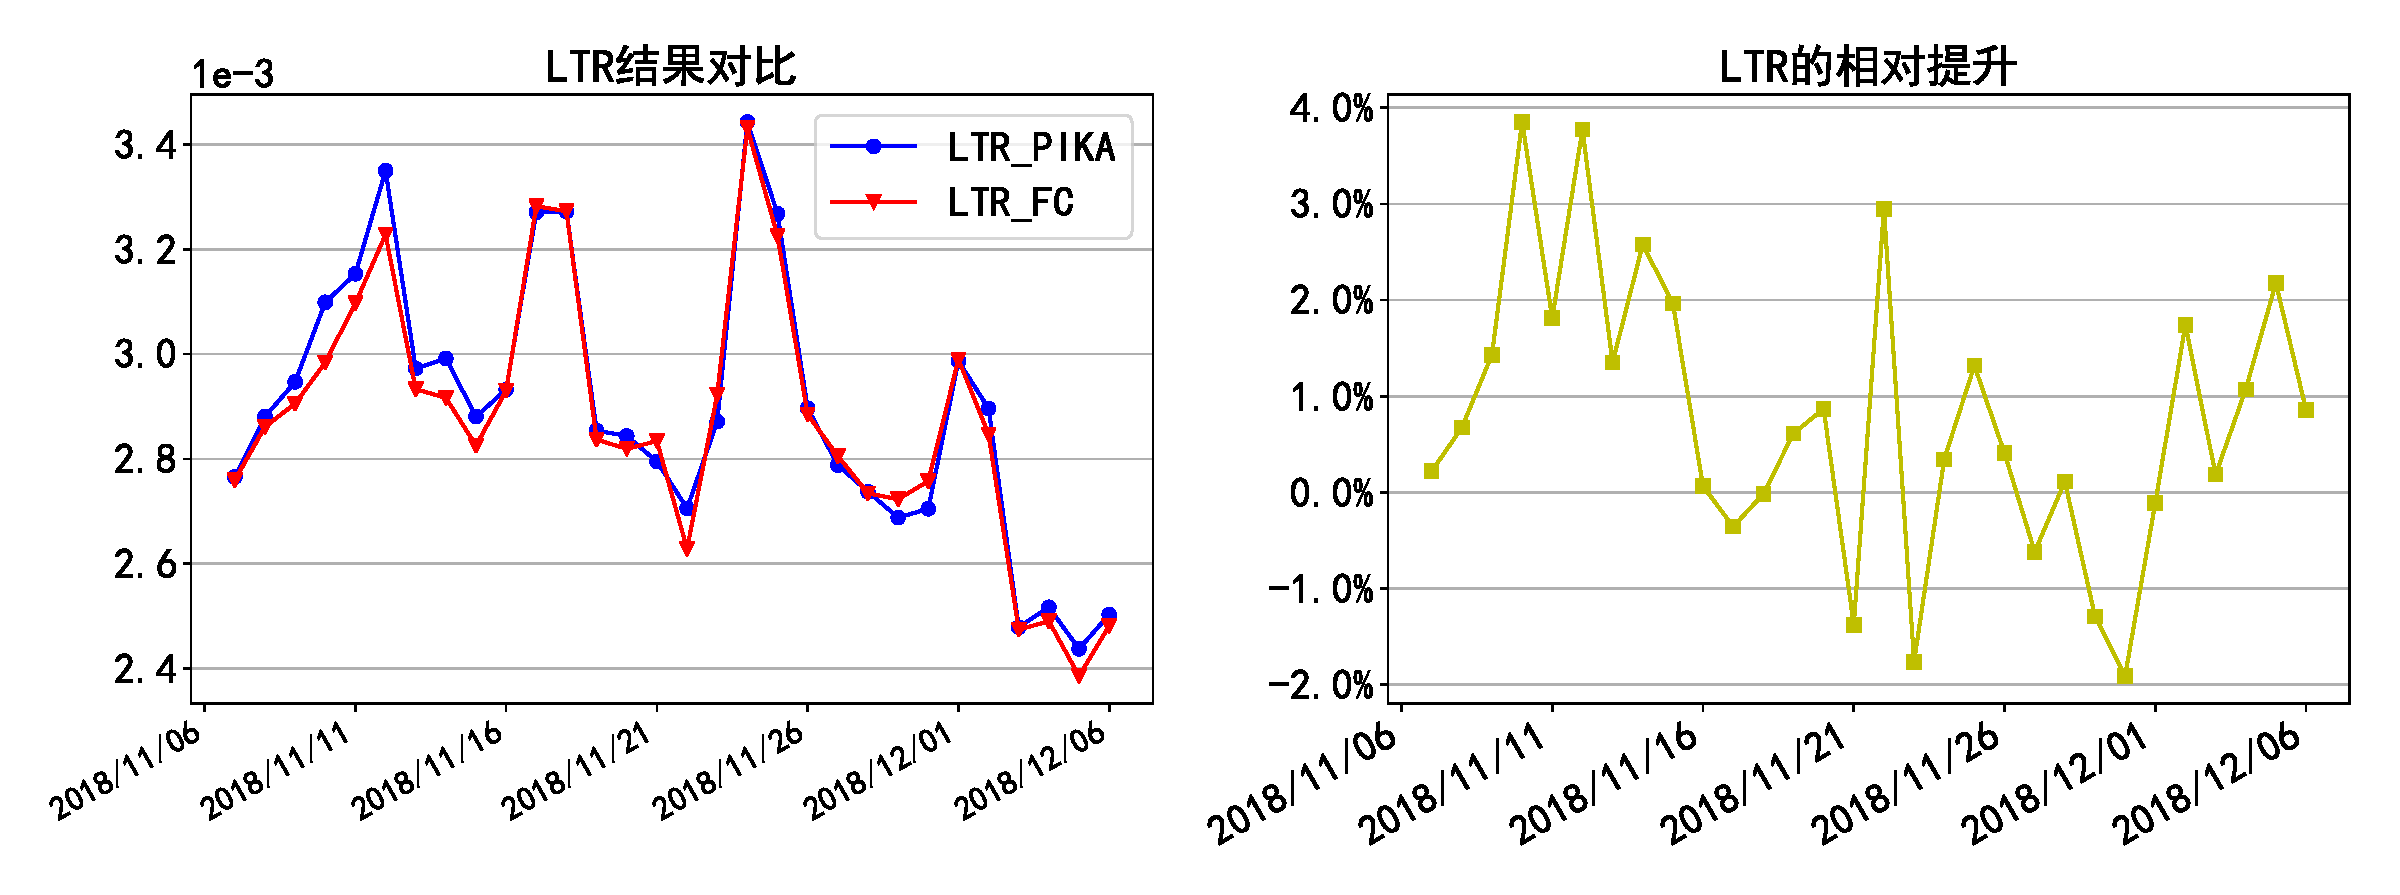
\includegraphics[width=\textwidth]{LTR.pdf}
	\caption{PIKA算法和FC在一个月内的LTR比较以及相对提升。LTR的表现与CTR类似,平均LTR的相对提升是$+0.752\%$}
	\label{fig:LTR}
\end{figure}

\begin{figure}[tb]
	\centering
	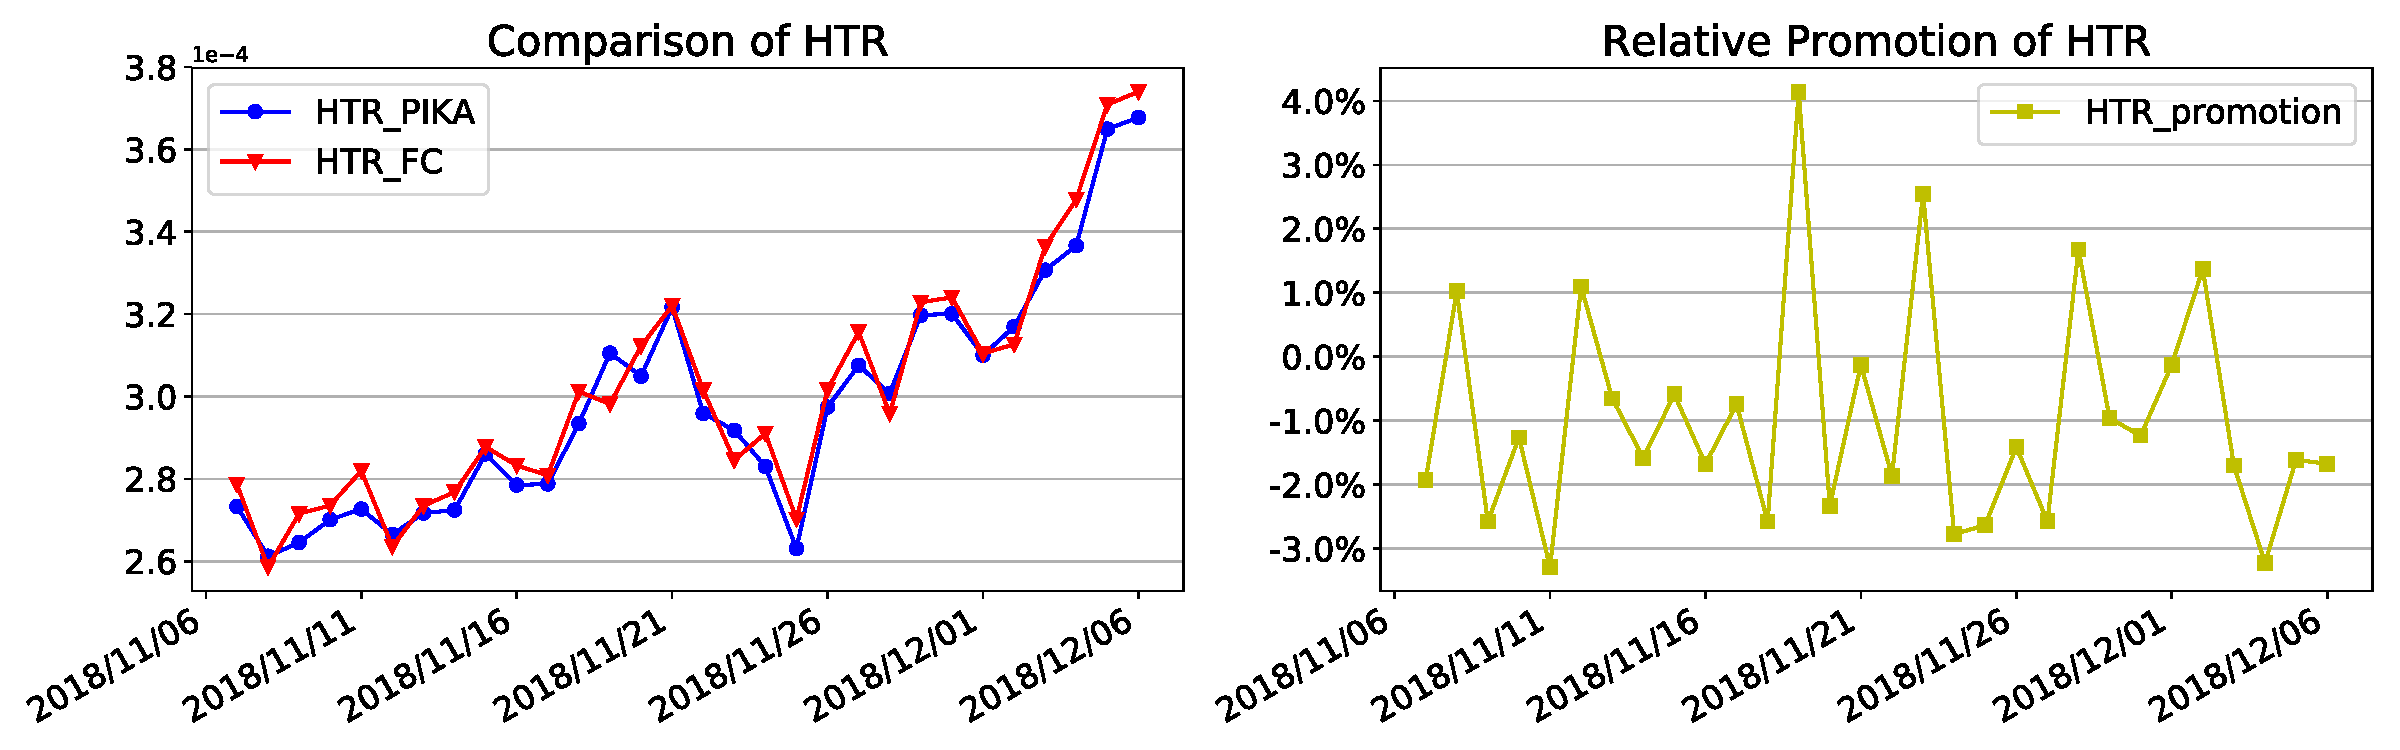
\includegraphics[width=\textwidth]{HTR.pdf}
	\caption{PIKA算法和FC在一个月内的HTR比较以及相对提升。不同于其他三个指标,HTR越低越好。这两条曲线相互交错,平均HTR的提升是$-1.10\%$。}
	\label{fig:HTR}
\end{figure}

\section{本章小结}

在本章,我们提出了一种最优广告投放算法PIKA以在保证广告主曝光量的情况下提升广告的投放效果。我们详细阐释了算法的数学原理,利用带约束优化问题的KKT条件给出一种高效的线上投放算法,并介绍一些工程实现上的细节。我们实现了该算法,同时进行了仿真实验,还在快手的同城页粉丝头条服务开展了线上A/B测试。仿真实验结果显示PIKA的投放量服从正态分布,佐证了曝光量保底策略的必要性,同时投放效果相比于简单贪心法获得了明显提升。线上实验表明,相比于快手原先部署的算法,PIKA在保证广告主曝光量的前提下,可以在最主要关心指标上取得更好的效果而在其他指标上持平。最终我们得出结论:PIKA算法的计算复杂度以及曝光量等性能指标达标,投放效果优于原先部署的流量控制算法。






